S\&G Soluciones de Ingeniería, una empresa enfocada en el desarrollo de proyectos de automatización, control, e implementación de soluciones tecnológicas industriales con un enfoque en IoT e industria 4.0. La empresa cuenta con más de 7 años de creación ha logrado anteponerse a las crisis económicas con la producida durante el periodo pandémico del 2019 y la reactivación post pandémica. Entre los años 2022 y 2024 (\Cref{fig:Cantidad de proyectos por país y año}), la empresa S\&G registró una tasa compuesta anual de crecimiento (CAGR) del 63.84\% en la ejecución de proyectos. Este indicador refleja un crecimiento sostenido y progresivo, mostrando una consolidación de su actividad operativa y un crecimiendo en sus operaciones a nivel regional, nacional e incursiones en el mercado internacional . Sin embargo, debido al crecimiento (\Cref{tab:Proyectos registrados por año}), ha enfrentado retos en la gestión de proyectos, principalmente por la falta de un marco estandarizado. 

\figuraConFuente{Cantidad de proyectos por país y año}
{
  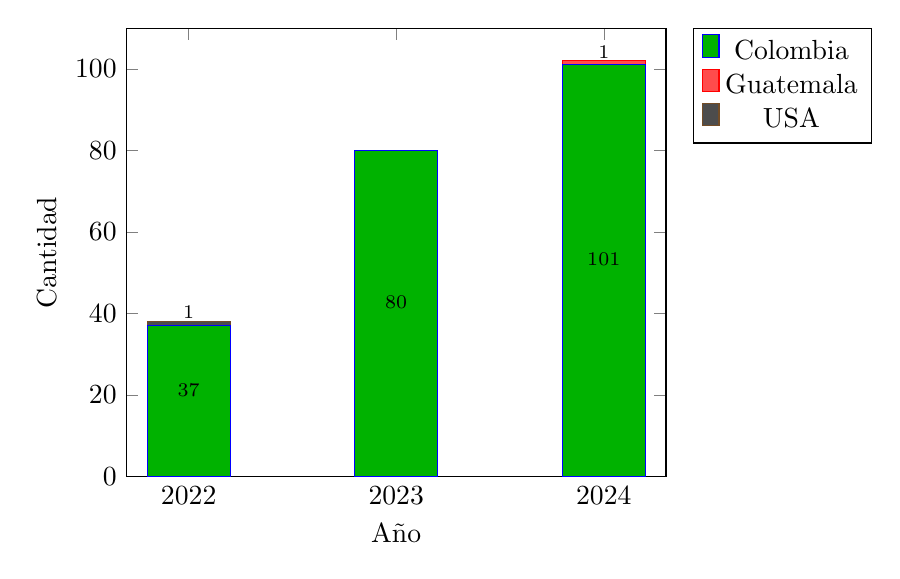
\begin{tikzpicture}
    \begin{axis}[
    ybar stacked,
  bar width=30pt,
  enlarge x limits=0.15,
  ymin=0,
  ymax=110,  % ajusta según necesidad
  xlabel={Año},
  ylabel={Cantidad},
  symbolic x coords={2022,2023,2024},
  xtick=data,
  legend style={at={(1.05,1)}, anchor=north west},
  ylabel near ticks,
  xlabel near ticks,
  nodes near coords,
  every node near coord/.append style={
    font=\scriptsize,
    color=black,
    yshift=4pt
  }
  ]

      \addplot+[fill=green!70!black] coordinates {
        (2022,37) (2023,80) (2024,101)
      };
      \addlegendentry{Colombia}

      \addplot+[fill=red!70] coordinates {
        (2022,0) (2023,0) (2024,1)
      };
      \addlegendentry{Guatemala}

      \addplot+[fill=black!70] coordinates {
        (2022,1) (2023,0) (2024,0)
      };
      \addlegendentry{USA}

    \end{axis}
  \end{tikzpicture}
}
{Elaboración propia basada en información interna (2025).}

\tablaConFuente{Proyectos registrados por año}{
  \begin{tabular}{ll}
    \toprule
    \textbf{Año} & \textbf{Total} \\
    \midrule
    2021 & 23 \\
    2022 & 38 \\
    2023 & 80 \\
    2024 & 102 \\
    \midrule
    \textbf{Total general} & \textbf{243} \\
    \bottomrule
  \end{tabular}
}{
  Elaboración propia basada en información interna (2025).
}

 De acuerdo con \parencite{kerznerUsingProjectManagement2019} La ausencia de un sistema claro provoca dificultades concretas, como la pérdida de control, problemas de gestión y complicaciones en la resolución eficiente de problemas con clientes, identificación insuficiente de las necesidades específicas en cada proyecto y administración ineficiente de los recursos disponibles. 

En este sentido y tomando en cuenta a \parencite{wysockiProjectManagementProcess2004} en la medida en que aumenta la demanda, los proyectos se vuelven mucho más complejos, los presupuestos mucho más rigurosos para administrar y también los riesgos crecen considerablemente. Teniendo en cuenta lo expuesto por \parencite{juhreManagingInternationalCrosscultural2000} Trabajar con clientes por fuera de Colombia implica también adaptarse a diferentes culturas administrativas y empresariales, lo que agrega otra capa más de complejidad. La falta de estandarización ha causado errores repetitivos, sobrecostos, retrasos y una potencial percepción negativa por parte de los clientes. 

Es fundamental implementar metodologías reconocidas internacionalmente, ofrecen un marco claro para establecer estrategias y sistematizar la gestión de proyectos, mejorar el uso de los recursos como también reducir los riesgos sobre tiempo y presupuesto. \parencite{projectmanagementinstituteStandardProjectManagement2021},\parencite{projectmanagementinstituteGuideProjectManagement2017},\parencite{associationforprojectmanagementAPMBodyKnowledge2019},\parencite{isoISO2150020212021}, Project Management by ICB4 \parencite{hedemanProjectManagementICB42023} y guías como la propuesta por \parencite{kerznerProjectManagementSystems2006}

Por otra parte, evaluar la madurez organizacional en gestión de proyectos, utilizando modelos como el OPM3® del PMI, permite identificar claramente fortalezas y debilidades actuales permitiendo establecer una ruta de mejora. Planear una implementación para la Oficina de Proyectos (OP) sería un paso estratégico adicional, que facilitaría la estandarización de los procesos y centralizaría el seguimiento de los proyectos.

Por otro lado, según la información proporcionada por (Confecámaras, 2024)las empresas dedicadas a la construcción, actividades profesionales, científicas y técnicas experimentaron un crecimiento del 47,5\% en el año 2023. Este crecimiento implica la creación de al menos un empleo por cada empresa establecida, esto que ratifica la relevancia estratégica del sector técnico y profesional en la economía colombiana.

En relación con lo anterior, estos datos son coherentes a lo planteado por González y Llanes (2024) en el informe Una mirada a las MiPymes en Colombia, en donde afirman que el 99,5\% del tejido empresarial colombiano está compuesto por micro, pequeñas y medianas empresas (MiPymes), las cuales aportan cerca del 40\% al Producto Interno Bruto (PIB) del país.

Según los datos previamente mencionados, implementar una metodología formal de gestión de proyectos y proponer un plan gradual para establecer una Oficina de Proyectos, representaría una estrategia adecuada frente a los desafíos actuales de S\&G Soluciones de Ingeniería. Estas medidas permitirían mejorar directamente la eficiencia, calidad y rentabilidad de los proyectos, creando así una base sólida para un crecimiento sostenido y competitivo dentro del sector tecnológico e industrial. 
